% id: 36-12
% book: 100발100중 3-2 기말 · 01 3-2 기말(원의 성질·통계·부록)
% section: 실전 문제 1회
% figure: crop:fig-36-12.png
% answer: $\angle x=95^\circ$, $\angle y=85^\circ$
% answer_source: 답지(빠른정답)
% variant_level: 0 (원본 전사)
% 이 파일은 build.mjs 가 items.json 에서 만든다. 고칠 때는 items.json 을 고친다.
\smash{\raisebox{1.5mm}{\dmkichul{100발100중 3-2 기말 36쪽 12번 · 출제유력 · 서술형}}}
\noindent\begin{minipage}[t]{0.58\linewidth}\vspace{0pt}\raggedright 그림과 같이 $\square\pt{ABCD}$가 원~$\pt{O}$에 내접하고 $\angle\pt{BAC}=35^\circ$, $\angle\pt{BCA}=50^\circ$일 때, $\angle x$, $\angle y$의 크기를 각각 구하고, 그 과정을 서술하시오. \mbox{[5점]}\end{minipage}\hfill\begin{minipage}[t]{0.4\linewidth}\vspace{0pt}\centering 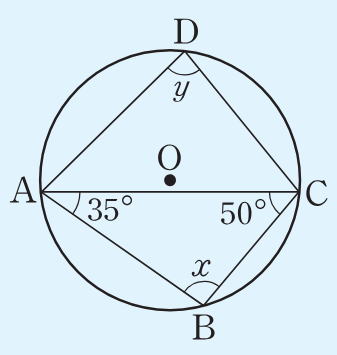
\includegraphics[width=80.7pt]{figures/fig-36-12.png}\end{minipage}\par
